\chapter{融合小波包分解的时频域增强方法}

本章的主要贡献在于，在第三章统一骨架上提出了一种面向多元长程时间序列预测的小波包多尺度增强方法，并将其系统地嵌入时频协同建模流程中。与基座模型中基于 FFT 幅值的轻量频域分支相比，本章首先通过小波包分解显式拆分不同频带的局部结构，使长期趋势、周期变化与高频突变能够在不同子带中分别建模\cite{mallat1989wavelet,coifman1992bestbasis,fan2008wavelet}。其次，本文为各子带设计了独立投影、频带身份编码、共享门控编码器和注意力池化机制，使模型不仅能够获取多尺度频带信息，还能够对不同子带的重要性进行自适应选择。最后，本章通过时域分支与小波包分支之间的跨注意力交互构建更细粒度的时频融合路径，为后续从机理层面解释其在 MSE 和极端波动场景下的优势奠定了结构基础\cite{vaswani2017attention,qiu2025gatedattention}。  

\section{问题分析与研究动机}

多元长程时间序列通常同时包含长期趋势、季节性波动、局部尖峰和突变噪声等多种成分。仅依赖时域编码器进行统一建模时，模型虽然能够学习整体动态模式，但对不同尺度成分的解耦能力有限，尤其在存在剧烈波动或局部异常点时，预测误差容易集中在少量时间步上。由于 MSE 对大误差样本具有平方放大效应，这类局部建模不足会直接拉高整体 MSE 指标\cite{hyndman2006accuracy,chai2014rmsemae}。  

与第五章将讨论的全局频域建模不同，小波包分解能够同时对低频与高频分量进行递归细分，从而得到一组具有明确频带含义的多尺度子带表示。与仅保留全局谱结构的傅里叶方法相比，该策略更适合描述局部时频变化，尤其适用于周期模式与突变行为并存的场景\cite{coifman1992bestbasis,tang2016timefreqwavelet}。对多元长程预测任务而言，这意味着模型可以先在频带层面对信号进行分解，再分别对不同子带进行编码和选择性融合，从而在保留长期趋势信息的同时增强对局部大偏差的抑制能力。  

基于上述考虑，本章在第三章统一骨架下，将频域分支具体替换为小波包增强模块，形成“时域编码 + 小波包多尺度建模 + 冻结语义先验 + 跨模态对齐”的完整模型\cite{kim2022revin,jiang2024empowering}。与原始基座相比，该模型的核心差异在于：频域信息不再由单一 FFT 幅值表示提供，而是通过多子带分解、逐子带编码、注意力池化与跨分支交互共同构成。由此，本章的研究目标可以概括为三个方面：给出小波包分解版本的具体结构设计；分析多尺度子带特征如何与时域特征及语义先验协同；通过实验验证该方法在 MSE 与极端波动场景下的优势。

\section{模型架构设计}

图\ref{fig:chap4-wavelet-packet-overview}给出了本章所提出的融合小波包分解的时频域增强模型整体结构。与第三章统一骨架相比，该模型将频域分支替换为可学习小波包分解模块，并在子带级编码、频带聚合以及步长感知融合的基础上与冻结语义先验共同完成预测\cite{coifman1992bestbasis,sweldens1997lifting,jiang2024empowering}。

\begin{figure}[!ht]
\centering
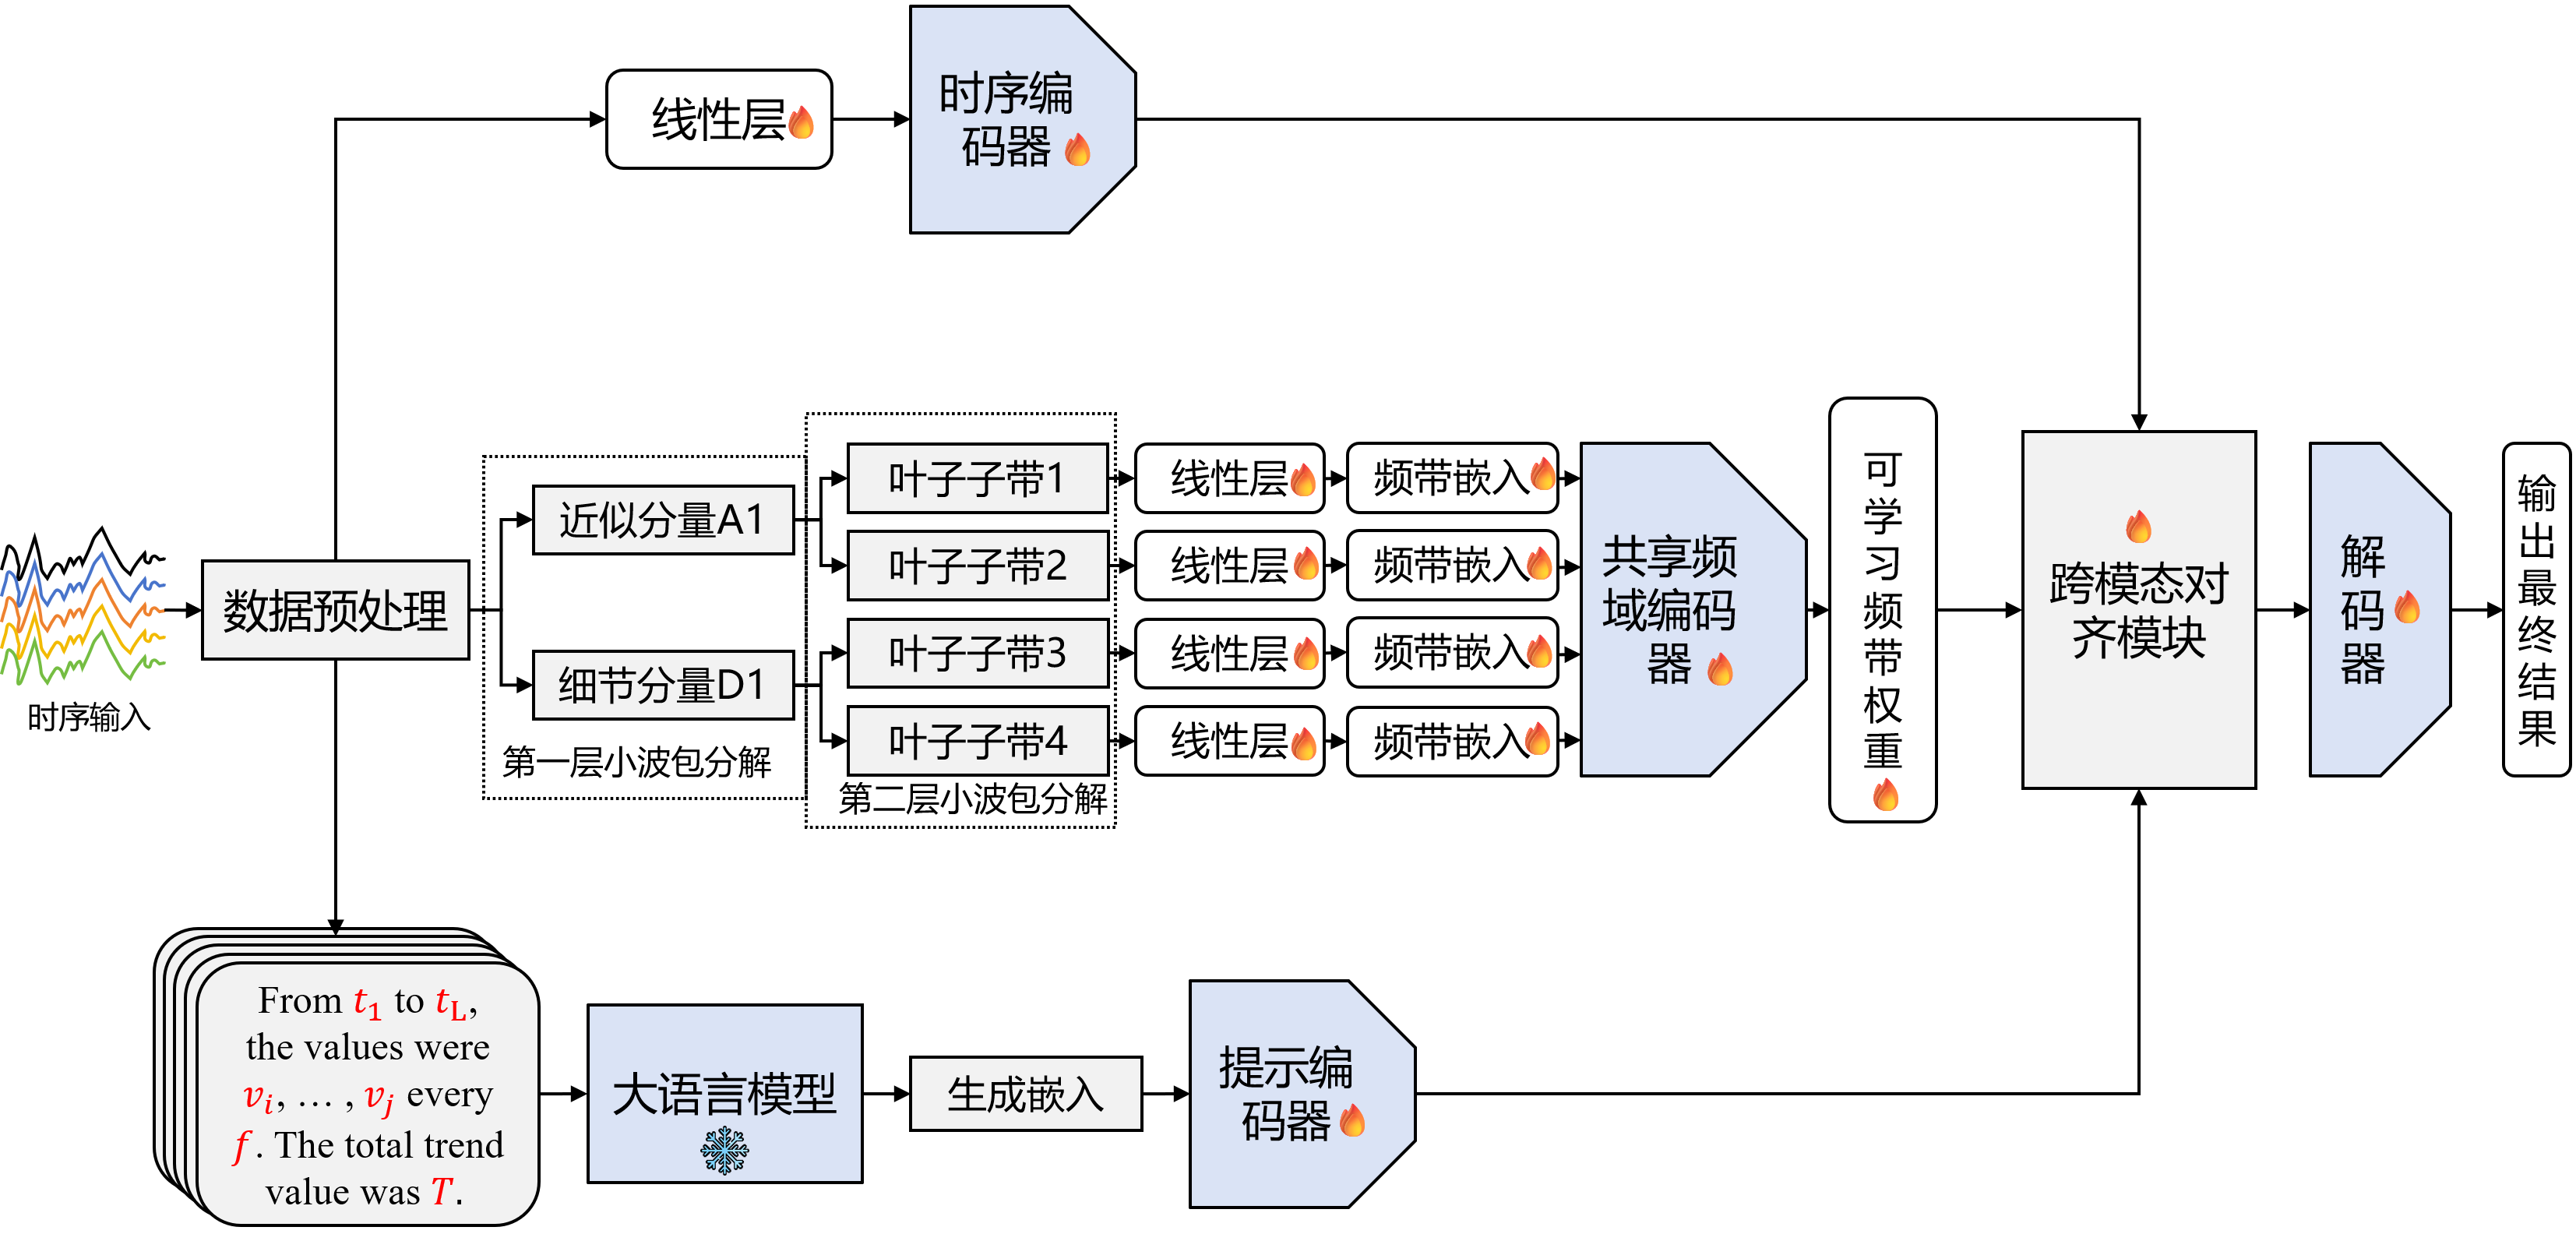
\includegraphics[width=\textwidth]{Img/chap4_wavelet_packet_overview.png}
\bicaption{融合小波包分解的时频域增强模型整体结构图}{Overall architecture of the time-frequency enhanced model with wavelet packet decomposition}
\label{fig:chap4-wavelet-packet-overview}
\end{figure}

\subsection{小波包多尺度分解策略}

本章的小波包增强模块建立在第三章统一骨架之上，但频域分支不再采用单一的 FFT 幅值表示，而是引入可学习小波包分解（learnable wavelet packet decomposition）对输入序列进行递归式多尺度拆分\cite{coifman1992bestbasis,sweldens1997lifting}。设经 RevIN 归一化后的输入序列为

\begin{figure}[!ht]
\centering
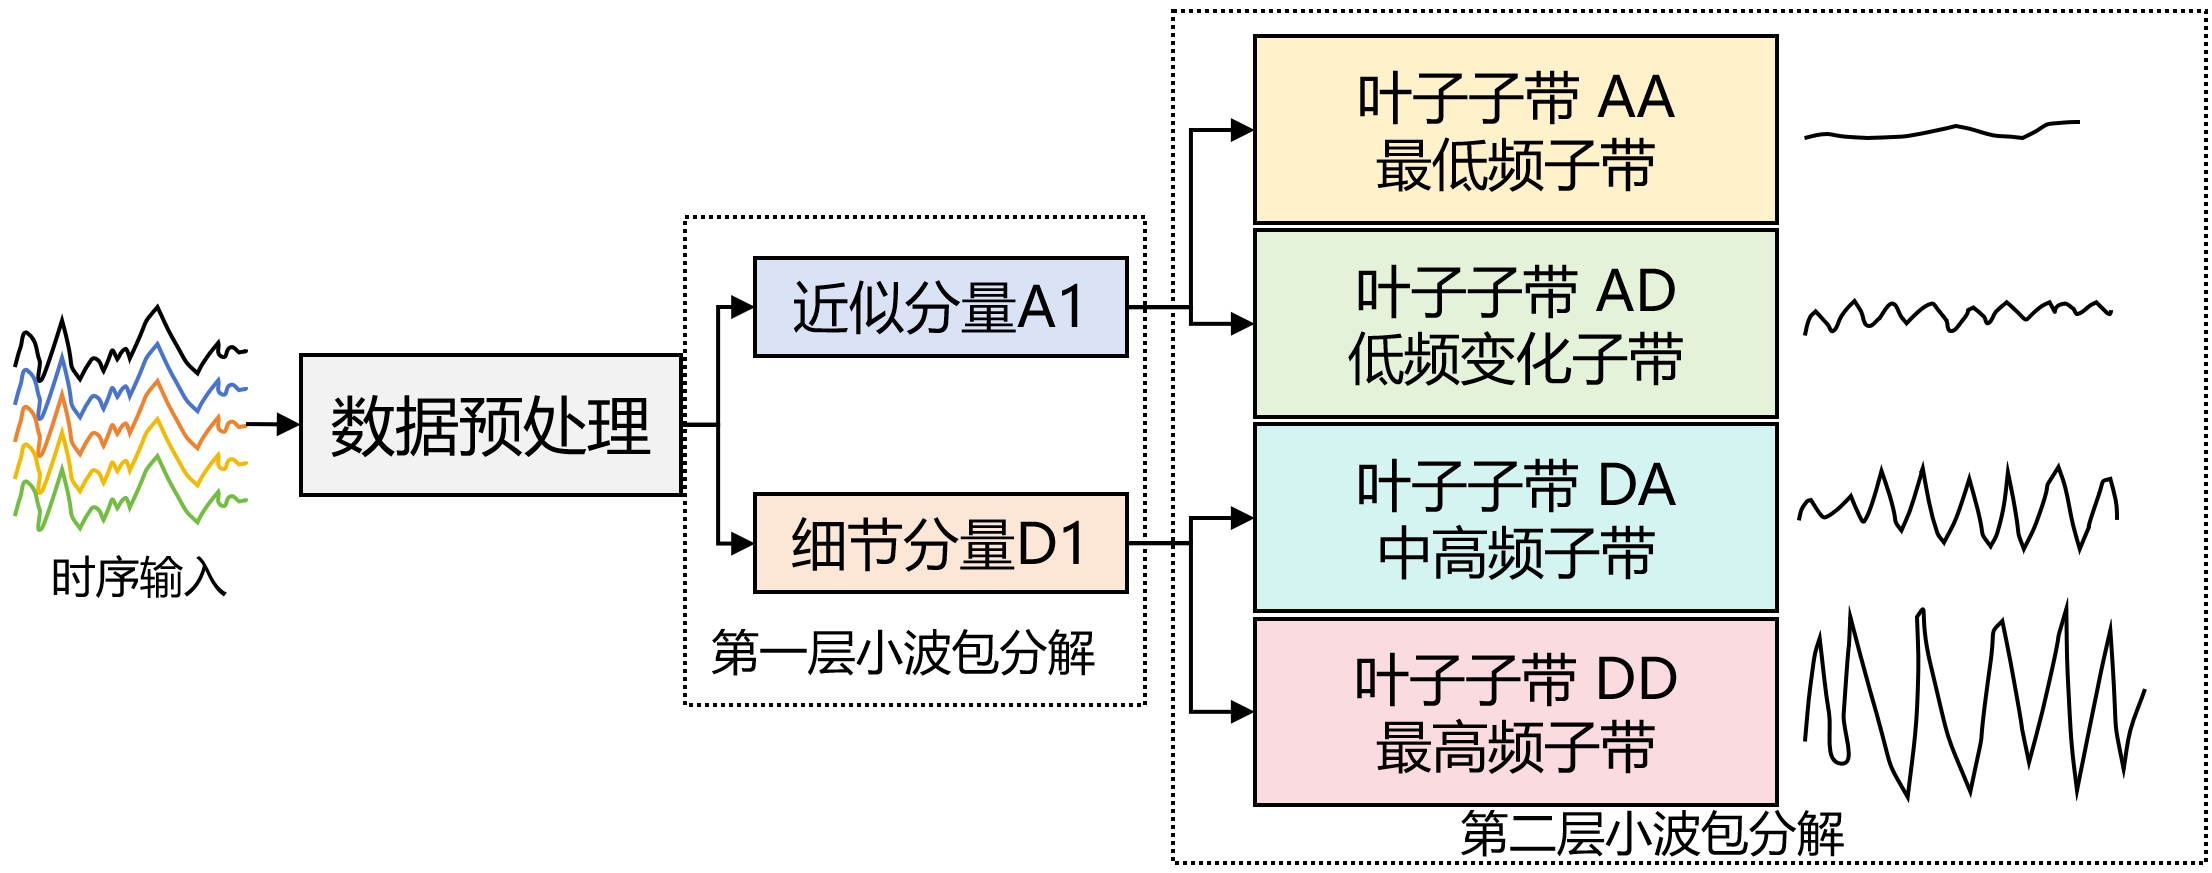
\includegraphics[width=\textwidth]{Img/chap4_wavelet_packet_decomposition.png}
\bicaption{两层小波包分解及叶子子带结构示意图}{Illustration of two-level wavelet packet decomposition and leaf subbands}
\label{fig:chap4-wavelet-packet-decomposition}
\end{figure}

图\ref{fig:chap4-wavelet-packet-decomposition}展示了本章采用的两层小波包分解过程。输入序列在第 1 层被拆分为近似分量和细节分量，随后两类分量在第 2 层继续递归分解，最终形成具有明确频带语义的 4 个叶子子带，为后续的子带级编码与频带聚合提供基础\cite{coifman1992bestbasis,fan2008wavelet}。

从频带语义上看，叶子子带 AA 对应最低频部分，主要保留序列中的长期趋势与缓慢变化成分；子带 AD 由近似分量继续分解得到，反映在总体平滑背景下的低频起伏与次级周期变化；子带 DA 对应中高频范围，更多刻画局部振荡、短期波动以及较快的周期扰动；子带 DD 则处于最高频区域，通常包含尖峰、突变、噪声和剧烈局部变化等细节信息。图中四条示意波形正是为了直观展示这种“由低频到高频、由平滑到剧烈”的变化规律。通过将不同频率层次的成分显式拆分，模型能够在后续编码过程中分别建模长期趋势、低频变化和高频扰动，从而提高对复杂非平稳时间序列的表达能力。

\noindent 设经 RevIN 归一化后的输入序列为
\begin{equation}
\mathbf{X}'\in\mathbb{R}^{B\times N\times L}
\label{eq:chap4-input}
\end{equation}
其中 \(B\) 表示批量大小，\(N\) 表示变量个数，\(L\) 表示历史窗口长度。对任意样本与变量索引 \((b,n)\)，记对应的一维时间序列为
\begin{equation}
\mathbf{x}^{(b,n)}=\bigl[x^{(b,n)}_1,x^{(b,n)}_2,\dots,x^{(b,n)}_L\bigr]^\top\in\mathbb{R}^{L}.
\label{eq:chap4-single-series}
\end{equation}
在实现上，所有变量序列先被展平为
\begin{equation}
\mathbf{X}_{\mathrm{flat}}\in\mathbb{R}^{BN\times 1\times L}
\label{eq:chap4-flat-series}
\end{equation}
从而能够对每个变量通道独立执行同构的小波包分解。与传统固定滤波器形式的小波包变换不同，本章采用提升格式（lifting scheme）构造可学习的小波包步骤\cite{sweldens1997lifting,tang2016timefreqwavelet}。设第 \(j\) 层第 \(k\) 个节点表示为 \(\mathbf{s}^{(j,k)}\in\mathbb{R}^{BN\times 1\times L_j}\)，其根节点满足
\begin{equation}
\mathbf{s}^{(0,1)}=\mathbf{X}_{\mathrm{flat}}.
\label{eq:chap4-root-node}
\end{equation}
对任意节点 \(\mathbf{s}^{(j,k)}\)，首先沿时间维执行奇偶拆分，得到
\begin{equation}
\mathbf{s}^{(j,k)}_{\mathrm{e}}=\mathbf{D}_{\mathrm{e}}^{(j)}\mathbf{s}^{(j,k)}
\label{eq:chap4-even}
\end{equation}
\begin{equation}
\mathbf{s}^{(j,k)}_{\mathrm{o}}=\mathbf{D}_{\mathrm{o}}^{(j)}\mathbf{s}^{(j,k)}
\label{eq:chap4-odd}
\end{equation}
其中 \(\mathbf{D}_{\mathrm{e}}^{(j)}\in\mathbb{R}^{\tilde{L}_j\times L_j}\) 与 \(\mathbf{D}_{\mathrm{o}}^{(j)}\in\mathbb{R}^{\tilde{L}_j\times L_j}\) 分别表示偶位与奇位下采样选择矩阵，满足
\begin{equation}
\bigl[\mathbf{D}_{\mathrm{e}}^{(j)}\bigr]_{t,\ell}=
\begin{cases}
1, & \ell=2t,\\
0, & \text{otherwise}
\end{cases}
\label{eq:chap4-even-matrix}
\end{equation}
\begin{equation}
\bigl[\mathbf{D}_{\mathrm{o}}^{(j)}\bigr]_{t,\ell}=
\begin{cases}
1, & \ell=2t+1,\\
0, & \text{otherwise}
\end{cases}
\label{eq:chap4-sampling-matrix}
\end{equation}
这里 \(\tilde{L}_j=\lfloor L_j/2 \rfloor\)。式（\ref{eq:chap4-even-matrix}）和式（\ref{eq:chap4-sampling-matrix}）中的 \(\mathbf{D}_{\mathrm{e}}^{(j)}\) 与 \(\mathbf{D}_{\mathrm{o}}^{(j)}\) 本质上是两类稀疏选择矩阵，其作用并不是引入额外可学习参数，而是以矩阵乘法的形式显式完成“抽取偶数位置样本”和“抽取奇数位置样本”这一步骤。换言之，\(\mathbf{D}_{\mathrm{e}}^{(j)}\mathbf{s}^{(j,k)}\) 保留节点序列中的第 \(0,2,4,\dots\) 个时间位置，而 \(\mathbf{D}_{\mathrm{o}}^{(j)}\mathbf{s}^{(j,k)}\) 保留第 \(1,3,5,\dots\) 个时间位置。  

为了便于理解，若暂不考虑批量维和通道维，并令 \(L_j=8\)，则节点序列 \(\mathbf{s}^{(j,k)}=[s_0,s_1,\dots,s_7]^\top\) 经过选择矩阵作用后可写为
\begin{equation}
\mathbf{D}_{\mathrm{e}}^{(j)}\mathbf{s}^{(j,k)}=
\begin{bmatrix}
s_0 & s_2 & s_4 & s_6
\end{bmatrix}^{\top}
\label{eq:chap4-even-example}
\end{equation}
\begin{equation}
\mathbf{D}_{\mathrm{o}}^{(j)}\mathbf{s}^{(j,k)}=
\begin{bmatrix}
s_1 & s_3 & s_5 & s_7
\end{bmatrix}^{\top}.
\label{eq:chap4-odd-example}
\end{equation}
因此，上述矩阵化表示只是将代码中“按步长为 2 的切片并截断到共同长度”的操作写成更严格的线性算子形式，其核心目的是为后续的预测算子和更新算子提供两路互补的子序列输入。随后分别利用可学习的预测算子 \(P_j(\cdot)\) 和更新算子 \(U_j(\cdot)\) 生成细节分量与近似分量：
\begin{equation}
\mathbf{d}^{(j,k)}=\mathbf{s}^{(j,k)}_{\mathrm{o}}-P_j\!\left(\mathbf{s}^{(j,k)}_{\mathrm{e}}\right)
\label{eq:chap4-detail}
\end{equation}
\begin{equation}
\mathbf{a}^{(j,k)}=\mathbf{s}^{(j,k)}_{\mathrm{e}}+U_j\!\left(\mathbf{d}^{(j,k)}\right).
\label{eq:chap4-approx}
\end{equation}
其中，\(P_j(\cdot)\) 与 \(U_j(\cdot)\) 在实现上均由两层一维卷积和 LeakyReLU 激活组成。若卷积核大小记为 3、隐藏通道数记为 8，则可形式化写为
\begin{equation}
P_j(\mathbf{z})=\mathbf{W}^{p,2}_j * \phi\!\left(\mathbf{W}^{p,1}_j * \mathbf{z}+\mathbf{b}^{p,1}_j\right)+\mathbf{b}^{p,2}_j
\label{eq:chap4-predict-op}
\end{equation}
\begin{equation}
U_j(\mathbf{z})=\mathbf{W}^{u,2}_j * \phi\!\left(\mathbf{W}^{u,1}_j * \mathbf{z}+\mathbf{b}^{u,1}_j\right)+\mathbf{b}^{u,2}_j
\label{eq:chap4-update-op}
\end{equation}
其中 \(*\) 表示一维卷积，\(\phi(\cdot)\) 表示 LeakyReLU 激活函数。与固定 \texttt{db4} 滤波器相比，该设计能够根据不同数据集的统计特征自动调整分解行为，因此更适合多元时间序列预测中的异质变量建模场景\cite{daubechies1992ten,sweldens1997lifting}。  

为了抑制局部噪声对子带分解的干扰，本章进一步在近似分量和细节分量上引入可学习软阈值函数\cite{donoho1994waveshrink}。对任意输入 \(z\)，其形式可写为
\begin{equation}
\mathcal{S}_{\tau}(z)=\mathrm{sign}(z)\max(|z|-\tau,0)
\label{eq:chap4-soft-threshold}
\end{equation}
其中 \(\tau\) 为可学习阈值参数。在实现中，近似分量与细节分量分别配置独立阈值 \(\tau_a,\tau_d\)。于是，式（\ref{eq:chap4-detail}）和式（\ref{eq:chap4-approx}）中的结果在进入下一层分解之前被修正为
\begin{equation}
\tilde{\mathbf{d}}^{(j,k)}=\mathcal{S}_{\tau_d}\!\left(\mathbf{d}^{(j,k)}\right)
\label{eq:chap4-threshold-detail}
\end{equation}
\begin{equation}
\tilde{\mathbf{a}}^{(j,k)}=\mathcal{S}_{\tau_a}\!\left(\mathbf{a}^{(j,k)}\right).
\label{eq:chap4-threshold-approx}
\end{equation}
该机制的作用在于削弱幅值较小且不稳定的局部扰动，使分解后的子带表示更加稀疏和稳健，也与后续实验中 MSE 对大误差样本的敏感性分析形成对应\cite{donoho1994waveshrink,chai2014rmsemae}。  

在小波包框架下，近似分量与细节分量都会继续向下递归分解。若分解层数设为 \(J\)，则对任意 \(j=0,1,\dots,J-1\) 和节点索引 \(k=1,\dots,2^j\)，其两个子节点递归定义为
\begin{equation}
\mathbf{s}^{(j+1,2k-1)}=\tilde{\mathbf{a}}^{(j,k)}
\label{eq:chap4-left-child}
\end{equation}
\begin{equation}
\mathbf{s}^{(j+1,2k)}=\tilde{\mathbf{d}}^{(j,k)}.
\label{eq:chap4-right-child}
\end{equation}
因此，第 \(j\) 层共有 \(2^j\) 个节点，第 \(J\) 层可得到 \(2^J\) 个叶子子带。记第 \(J\) 层第 \(i\) 个叶子节点为 \(\mathbf{S}_i\in\mathbb{R}^{B\times N\times L_i}\)，则有
\begin{equation}
\mathbf{S}_i=\operatorname{Reshape}\!\left(\mathbf{s}^{(J,i)}\right)
\label{eq:chap4-wpd}
\end{equation}
\begin{equation}
i\in\{1,2,\dots,2^J\}
\label{eq:chap4-wpd-index}
\end{equation}
\begin{equation}
\mathcal{S}^{(J)}=\{\mathbf{S}_1,\mathbf{S}_2,\dots,\mathbf{S}_{2^J}\}.
\label{eq:chap4-wpd-set}
\end{equation}
其中 \(L_i\approx L/2^J\)。在本文默认设置中取 \(J=2\)，因此最终可以得到 4 个叶子子带，分别记为 AA、AD、DA 和 DD。这样的设置兼顾了频带分辨率与子带长度：若 \(J\) 过小，则不同尺度成分无法充分分离；若 \(J\) 过大，则子带长度过短，局部表示容易变得不稳定，并增加后续建模开销\cite{coifman1992bestbasis,fan2008wavelet}。  

从建模机制上看，式（\ref{eq:chap4-left-child})--式（\ref{eq:chap4-wpd-set}）并不是简单地增加特征数量，而是将原始时间序列中耦合在一起的低频趋势、周期波动与高频扰动递归拆解为多路具有明确频带含义的子序列。由此，模型可以在子带层面分别学习局部模式，再在后续阶段完成重组与融合。这一结构正是第四章区别于第三章统一骨架以及第五章全局频域前馈方案的关键所在。

\subsection{频域子带特征与 LLM 嵌入空间的映射机制}

得到 \(\{\mathbf{S}_i\}_{i=1}^{2^J}\) 后，模型需要将不同长度的子带映射到统一的通道空间，以便后续与时域分支和语义分支对齐。为此，本文为每个叶子子带配置独立的线性投影层 \(\mathbf{W}_i\in\mathbb{R}^{1\times C}\)。将第 \(i\) 个子带重排为 \(\mathbf{Z}_i\in\mathbb{R}^{BN\times L_i\times 1}\) 后，其初始嵌入形式可写为
\begin{equation}
\mathbf{Z}_i=\operatorname{Transpose}\!\left(\mathbf{S}_i\right)
\label{eq:chap4-band-reshape}
\end{equation}
\begin{equation}
\mathbf{H}_i^{(0)}=\mathbf{Z}_i\mathbf{W}_i+\mathbf{1}_{L_i}\mathbf{b}_i^\top
\label{eq:chap4-band-proj}
\end{equation}
\begin{equation}
\mathbf{H}_i^{(0)}\in\mathbb{R}^{BN\times L_i\times C}
\label{eq:chap4-band-proj-shape}
\end{equation}
其中 \(C\) 为统一通道维度。使用独立投影而非共享投影的原因在于，不同子带对应的频谱区域和统计特性并不相同，单一线性映射难以同时兼顾低频趋势与高频扰动的表达需求。  

为了在参数共享的后续编码过程中保留“频带身份”，本章进一步为每个子带引入可学习的频带身份嵌入 \(\mathbf{e}_i\in\mathbb{R}^{C}\)。令 \(\mathbf{E}_i=\mathbf{1}_{L_i}\mathbf{e}_i^\top\in\mathbb{R}^{L_i\times C}\) 表示沿时间维复制后的频带嵌入矩阵，则有
\begin{equation}
\mathbf{H}_i^{(1)}=\mathbf{H}_i^{(0)}+\mathbf{E}_i.
\label{eq:chap4-band-id}
\end{equation}
这里的嵌入并非时间位置编码，而是对子带语义的显式标识，旨在让共享编码器能够区分“当前特征来源于哪个频段”。随后，所有子带特征共享同一个门控 Transformer 编码器进行建模\cite{vaswani2017attention,qiu2025gatedattention}。若记编码器为 \(\mathcal{E}_{\mathrm{wp}}(\cdot)\)，则有
\begin{equation}
\tilde{\mathbf{H}}_i=\mathcal{E}_{\mathrm{wp}}\!\left(\mathbf{H}_i^{(1)}\right)
\label{eq:chap4-band-encoder}
\end{equation}
其中 \(\tilde{\mathbf{H}}_i\in\mathbb{R}^{BN\times L_i\times C}\)。若以单层编码器为例，其内部可进一步抽象为
\begin{equation}
\widehat{\mathbf{H}}_i=\operatorname{MHA}\!\left(\operatorname{LN}(\mathbf{H}_i^{(1)})\right)
\label{eq:chap4-shared-encoder-attn}
\end{equation}
\begin{equation}
\mathbf{G}_i=\sigma\!\left(\operatorname{LN}(\mathbf{H}_i^{(1)})\mathbf{W}_g+\mathbf{b}_g\right)
\label{eq:chap4-shared-encoder-gate}
\end{equation}
\begin{equation}
\mathbf{H}_i^{\mathrm{att}}=\mathbf{H}_i^{(1)}+\widehat{\mathbf{H}}_i\odot \mathbf{G}_i
\label{eq:chap4-shared-encoder-res}
\end{equation}
\begin{equation}
\tilde{\mathbf{H}}_i=\mathbf{H}_i^{\mathrm{att}}+\operatorname{FFN}\!\left(\operatorname{LN}(\mathbf{H}_i^{\mathrm{att}})\right)
\label{eq:chap4-shared-encoder-ffn}
\end{equation}
其中 \(\operatorname{MHA}(\cdot)\) 表示多头自注意力，\(\operatorname{LN}(\cdot)\) 表示层归一化，\(\odot\) 表示逐元素乘法。共享编码器一方面能够减少参数规模，另一方面也促使不同频带在统一表示空间中接受一致的建模约束。  

在获得时序编码结果后，模型需要进一步将每个子带压缩为变量级向量。本文采用注意力池化而非简单均值池化。设可学习查询向量为 \(\mathbf{q}\in\mathbb{R}^{C}\)，并记 \(\mathbf{Q}=\mathbf{1}_{BN}\mathbf{q}^\top\in\mathbb{R}^{BN\times C}\)，则第 \(i\) 个子带的注意力打分向量可写为
\begin{equation}
\mathbf{r}_i=\tilde{\mathbf{H}}_i\mathbf{q}\in\mathbb{R}^{BN\times L_i}
\label{eq:chap4-band-score}
\end{equation}
\begin{equation}
\boldsymbol{\alpha}_i=\operatorname{softmax}\!\left(\mathbf{r}_i\right)\in\mathbb{R}^{BN\times L_i}
\label{eq:chap4-band-attn}
\end{equation}
其中 softmax 沿时间维执行归一化。相应的变量级子带表示为
\begin{equation}
\mathbf{p}_i=\tilde{\mathbf{H}}_i^\top \boldsymbol{\alpha}_i \in \mathbb{R}^{BN\times C}.
\label{eq:chap4-band-pool}
\end{equation}
由此可得到所有子带的堆叠表示
\begin{equation}
\mathbf{P}=\operatorname{Stack}(\mathbf{p}_1,\dots,\mathbf{p}_{2^J})
\in\mathbb{R}^{BN\times 2^J\times C}
\label{eq:chap4-band-stack}
\end{equation}

在训练阶段，为避免模型过度依赖某一固定频带，代码实现中还引入了频带随机丢弃（frequency dropout）策略\cite{srivastava2014dropout}。若记随机掩码矩阵为 \(\mathbf{M}\in\{0,1\}^{BN\times 2^J\times 1}\)，则训练期输入可写为
\begin{equation}
\mathbf{P}^{\mathrm{drop}}=\mathbf{M}\odot \mathbf{P}
\label{eq:chap4-band-dropout}
\end{equation}
其中 \(\odot\) 表示逐元素乘法。推理阶段令 \(\mathbf{M}\equiv \mathbf{1}\)，从而恢复完整频带集合。进一步地，模型对所有子带向量执行一次频带级自注意力交互，以建模不同频带之间的相关性。若记该交互模块为 \(\mathcal{A}_{\mathrm{band}}(\cdot)\)，则有
\begin{equation}
\widehat{\mathbf{P}}=\mathcal{A}_{\mathrm{band}}\!\left(\mathbf{P}^{\mathrm{drop}}\right)\in\mathbb{R}^{BN\times 2^J\times C}
\label{eq:chap4-band-interaction}
\end{equation}
其第 \(i\) 个频带向量记为 \(\hat{\mathbf{p}}_i\in\mathbb{R}^{BN\times C}\)。若以单层频带级自注意力为例，则有
\begin{equation}
\mathbf{Q}_{\mathrm{band}}=\widehat{\mathbf{P}}\mathbf{W}_Q,\quad
\mathbf{K}_{\mathrm{band}}=\widehat{\mathbf{P}}\mathbf{W}_K,\quad
\mathbf{V}_{\mathrm{band}}=\widehat{\mathbf{P}}\mathbf{W}_V
\label{eq:chap4-band-qkv}
\end{equation}
\begin{equation}
\mathbf{A}_{\mathrm{band}}=\operatorname{softmax}\!\left(
\frac{\mathbf{Q}_{\mathrm{band}}\mathbf{K}_{\mathrm{band}}^\top}{\sqrt{d_c}}
\right)
\label{eq:chap4-band-attn-mat}
\end{equation}
\begin{equation}
\widehat{\mathbf{P}}=\mathbf{A}_{\mathrm{band}}\mathbf{V}_{\mathrm{band}}
\label{eq:chap4-band-attn-out}
\end{equation}
其中 \(d_c\) 表示每个注意力头的通道维度。随后，引入具有先验初始化的可学习频带权重 \(\mathbf{w}_i\in\mathbb{R}^{C}\)，并定义
\begin{equation}
\boldsymbol{\beta}_i=\sigma(\mathbf{w}_i)\in(0,1)^C
\label{eq:chap4-band-weight}
\end{equation}
最终的小波包分支表示为
\begin{equation}
\mathbf{H}^{\mathrm{wp}}
=\sum_{i=1}^{2^J}\boldsymbol{\beta}_i\odot \hat{\mathbf{p}}_i
\label{eq:chap4-wp-final}
\end{equation}
其中 \(\sigma(\cdot)\) 为 Sigmoid 函数。式（\ref{eq:chap4-band-dropout})--式（\ref{eq:chap4-wp-final}）表明，小波包分支并非对各叶子子带做简单拼接，而是先通过随机屏蔽提升鲁棒性，再通过频带级自注意力显式建模跨频带依赖关系，最后由可学习权重自适应决定不同频带对最终预测任务的贡献比例。  

需要指出的是，小波包分支并不直接与 LLM 的 token 级表示逐点对齐，而是先在本分支内部完成“分解、编码、池化、重组”，最终输出变量级表示 \(\mathbf{H}^{\mathrm{wp}}\in\mathbb{R}^{B\times N\times C}\)。这一设计使该分支能够自然地接入第三章的统一多模态框架，并在保持结构紧凑的同时降低跨模态对齐的复杂度\cite{jiang2024empowering,jin2024timellm}。

\subsection{多尺度特征融合与预测头设计}

与小波包分支并行，第三章中的时域主干仍然保留。对归一化后的输入 \(\mathbf{X}'\)，模型首先通过长度到特征的线性映射得到时域表示\cite{kim2022revin,vaswani2017attention}
\begin{equation}
\mathbf{H}^{\mathrm{time}}=\phi(\mathbf{X}')\in\mathbb{R}^{B\times N\times C}
\label{eq:chap4-time-branch}
\end{equation}
再经若干层门控 Transformer 编码器获得更高层时域特征。第四章的关键并不在于替换整个主干，而在于通过小波包分支为该主干提供局部多尺度补充信息\cite{vaswani2017attention,qiu2025gatedattention}。  

在时域与小波包分支的融合阶段，本文没有采用简单拼接，而是设计了显式的步长感知门控融合机制\cite{qiu2025gatedattention}。设预测步长归一化后形成的任务先验为 \(\mathbf{r}\in\mathbb{R}^{B\times N\times 1}\)，则融合门控可写为
\begin{equation}
\mathbf{G}
=\sigma\!\left(
\mathrm{MLP}\left[
\mathbf{H}^{\mathrm{time}};\
\mathbf{H}^{\mathrm{wp}};\
\mathbf{r}
\right]\right)
\label{eq:chap4-fusion-gate}
\end{equation}
其中 \([\cdot;\cdot;\cdot]\) 表示沿特征维拼接。最终融合结果为
\begin{equation}
\mathbf{H}^{\mathrm{fuse}}
=\mathbf{H}^{\mathrm{time}}+\mathbf{G}\odot\mathbf{H}^{\mathrm{wp}}.
\label{eq:chap4-fusion}
\end{equation}
式（\ref{eq:chap4-fusion}）说明，小波包分支不是对时域分支的简单替代，而是作为与预测跨度相关的残差增强项注入主干表示。这一机制使模型能够根据任务难度与步长尺度动态调整局部频带信息的注入强度。  

完成时频融合后，模型继续沿用第三章的统一语义增强流程。冻结大语言模型生成的变量级语义嵌入先经过 \texttt{prompt\_encoder} 编码，得到语义先验 \(\mathbf{H}^{\mathrm{sem}}\)。然后，融合后的时频表示与语义先验在 CMA 模块中执行跨模态对齐\cite{jiang2024empowering,jin2024timellm,zhang2025llmpowercn}：
\begin{equation}
\mathbf{H}^{\mathrm{cma}}
=\mathrm{CMA}\!\left(
\mathbf{H}^{\mathrm{fuse}},\
\mathbf{H}^{\mathrm{sem}},\
\mathbf{H}^{\mathrm{sem}}
\right).
\label{eq:chap4-cma}
\end{equation}
在此基础上，模型将 \(\mathbf{H}^{\mathrm{cma}}\) 输入解码器，并通过线性映射将通道维投影到预测步长维，得到最终预测输出：
\begin{equation}
\hat{\mathbf{Y}}
=\mathrm{Proj}\!\left(
\mathrm{Decoder}\left(\mathbf{H}^{\mathrm{cma}}\right)
\right)
\in\mathbb{R}^{B\times L_{\mathrm{pred}}\times N}.
\label{eq:chap4-output}
\end{equation}
最后，再通过 RevIN 的反归一化步骤恢复到原始数值尺度\cite{kim2022revin}。  

综合来看，第四章模型可以概括为“归一化输入 $\rightarrow$ 可学习小波包分解 $\rightarrow$ 子带级编码与池化 $\rightarrow$ 步长感知门控融合 $\rightarrow$ 语义对齐与解码预测”的五阶段流程。其中，小波包分支负责显式建模局部多尺度结构，时域主干负责保留原始时间依赖，语义分支负责补充变量层面的外部先验，而门控融合与 CMA 则承担不同模态之间的协同建模任务。该结构既继承了第三章统一骨架的整体稳定性，又通过局部多尺度分解机制增强了对尖峰、突变和高波动片段的刻画能力\cite{sweldens1997lifting,qiu2025gatedattention,jiang2024empowering}。

\section{实验设置与结果分析}

\subsection{实验设置与对比基线}

本章实验沿用第 3.4.1 节的基本设置，并保持数据集划分、输入窗口长度、预测长度和评价指标一致，以保证对比结果的公平性。模型方面，仅将统一框架中的频域分支替换为本章提出的小波包增强模块，其余部分如时域分支、语义分支、CMA 与解码器均保持不变。默认情况下，小波基选用 \texttt{db4}，分解层数设置为 2，对应 4 个叶子子带；损失函数可继续采用与总体实验一致的优化目标，并在结果展示阶段重点分析 MSE 指标\cite{daubechies1992ten,hyndman2006accuracy,chai2014rmsemae}。  

为了更清晰地体现小波包分支的实际贡献，本章设置了两组主对比实验。第一组基线包括 T3time、TimeCMA、TimeLLM 和 TimesNet，用于比较本章方法与统一框架、跨模态增强方法以及经典时序骨干之间的差异；第二组基线包括 UniTime、DLinear、iTransformer 和 PatchTST，用于补充统一建模、线性建模与 Transformer 路线下的强基线对照\cite{yi2023frets,zhou2022fedformer}。训练过程使用统一的优化器、学习率、batch size 和早停策略，以保证不同模型之间的比较具有公平性。

\subsection{MSE 指标表现及显著性分析}

本节重点考察小波包增强模型在 MSE 指标上的表现，并将结果与统一框架基线以及其他代表性长程预测方法进行比较。为与第五章主结果表的组织方式保持一致，表\ref{tab:chap4-main-results-a}和表\ref{tab:chap4-main-results-b}均按照“完整数据集 + 完整预测长度 + 共享 Ours 列”的形式重排：表\ref{tab:chap4-main-results-a}展示 Ours 与 T3time、TimeCMA、TimeLLM、TimesNet 的对比，表\ref{tab:chap4-main-results-b}展示 Ours 与 UniTime、DLinear、iTransformer、PatchTST 的对比。这样既便于后续直接回填完整实验结果，也便于与第五章两张主结果表进行横向对照。两张表同时保留 MSE 和 MAE 指标，其中本章后续分析仍以 MSE 为主，以突出小波包多尺度分解对大误差样本的抑制能力\cite{hyndman2006accuracy,chai2014rmsemae}。

\begin{table}[!htbp]
\centering
\small
\setlength{\tabcolsep}{3.6pt}
\renewcommand{\arraystretch}{0.96}
\bicaption{小波包分解增强方法的预测性能对比（1）}{Performance comparison of the wavelet packet decomposition enhanced method (1)}
\label{tab:chap4-main-results-a}
\begin{tabular}{c|c|cc|cc|cc|cc|cc}
\toprule
\multirow{2}{*}{\textbf{Dataset}} & \multirow{2}{*}{\textbf{Horizon}} &
\multicolumn{2}{c|}{\textbf{Ours}} &
\multicolumn{2}{c|}{\textbf{T3time}} &
\multicolumn{2}{c|}{\textbf{TimeCMA}} &
\multicolumn{2}{c|}{\textbf{TimeLLM}} &
\multicolumn{2}{c}{\textbf{TimesNet}} \\
& & MSE & MAE & MSE & MAE & MSE & MAE & MSE & MAE & MSE & MAE \\
\midrule
\multirow{5}{*}{ETTm1}
& 96 & \textbf{0.312} & 0.358 & \textbf{\textcolor{red}{0.308}} & \textbf{0.354} & \textbf{0.312} & \textbf{\textcolor{red}{0.351}} & 0.359 & 0.381 & 0.338 & 0.375 \\
& 192 & 0.365 & \textbf{0.379} & \textbf{\textcolor{red}{0.357}} & 0.381 & \textbf{0.361} & \textbf{\textcolor{red}{0.378}} & 0.383 & 0.393 & 0.374 & 0.387 \\
& 336 & 0.398 & 0.404 & \textbf{\textcolor{red}{0.382}} & \textbf{\textcolor{red}{0.400}} & \textbf{0.392} & \textbf{0.401} & 0.416 & 0.414 & 0.410 & 0.411 \\
& 720 & 0.468 & 0.441 & \textbf{\textcolor{red}{0.442}} & \textbf{\textcolor{red}{0.437}} & \textbf{0.453} & \textbf{0.438} & 0.483 & 0.449 & 0.478 & 0.450 \\
& Avg & 0.386 & 0.396 & \textbf{\textcolor{red}{0.372}} & \textbf{0.393} & \textbf{0.380} & \textbf{\textcolor{red}{0.392}} & 0.410 & 0.409 & 0.400 & 0.406 \\
\midrule
\multirow{5}{*}{ETTm2}
& 96 & \textbf{\textcolor{red}{0.170}} & \textbf{\textcolor{red}{0.251}} & \textbf{0.172} & \textbf{0.254} & 0.173 & 0.258 & 0.193 & 0.280 & 0.187 & 0.267 \\
& 192 & \textbf{\textcolor{red}{0.235}} & \textbf{\textcolor{red}{0.297}} & \textbf{0.237} & \textbf{0.300} & 0.238 & 0.301 & 0.257 & 0.318 & 0.249 & 0.309 \\
& 336 & \textbf{0.302} & \textbf{\textcolor{red}{0.334}} & 0.306 & \textbf{0.337} & \textbf{\textcolor{red}{0.297}} & 0.338 & 0.317 & 0.353 & 0.319 & 0.351 \\
& 720 & \textbf{0.396} & \textbf{\textcolor{red}{0.394}} & 0.400 & \textbf{0.398} & \textbf{\textcolor{red}{0.393}} & \textbf{\textcolor{red}{0.394}} & 0.419 & 0.411 & 0.408 & 0.403 \\
& Avg & \textbf{0.276} & \textbf{\textcolor{red}{0.319}} & 0.279 & \textbf{0.322} & \textbf{\textcolor{red}{0.275}} & 0.323 & 0.296 & 0.340 & 0.291 & 0.333 \\
\midrule
\multirow{5}{*}{ETTh1}
& 96 & \textbf{\textcolor{red}{0.370}} & \textbf{0.395} & \textbf{0.371} & 0.397 & 0.373 & \textbf{\textcolor{red}{0.391}} & 0.398 & 0.410 & 0.384 & 0.402 \\
& 192 & \textbf{0.419} & \textbf{0.423} & \textbf{\textcolor{red}{0.411}} & \textbf{\textcolor{red}{0.421}} & 0.427 & \textbf{\textcolor{red}{0.421}} & 0.451 & 0.440 & 0.434 & 0.429 \\
& 336 & 0.465 & \textbf{\textcolor{red}{0.440}} & \textbf{\textcolor{red}{0.448}} & \textbf{0.441} & \textbf{0.458} & 0.448 & 0.473 & 0.451 & 0.491 & 0.469 \\
& 720 & 0.455 & \textbf{0.462} & \textbf{\textcolor{red}{0.441}} & \textbf{\textcolor{red}{0.460}} & \textbf{0.449} & \textbf{\textcolor{red}{0.460}} & 0.469 & 0.470 & 0.521 & 0.500 \\
& Avg & 0.427 & \textbf{\textcolor{red}{0.430}} & \textbf{\textcolor{red}{0.418}} & \textbf{\textcolor{red}{0.430}} & \textbf{0.423} & \textbf{0.431} & 0.448 & 0.443 & 0.458 & 0.450 \\
\midrule
\multirow{5}{*}{ETTh2}
& 96 & \textbf{\textcolor{red}{0.277}} & \textbf{\textcolor{red}{0.332}} & \textbf{0.278} & 0.338 & 0.286 & \textbf{0.336} & 0.295 & 0.345 & 0.340 & 0.374 \\
& 192 & \textbf{\textcolor{red}{0.351}} & \textbf{\textcolor{red}{0.385}} & \textbf{\textcolor{red}{0.351}} & 0.389 & \textbf{0.363} & \textbf{0.387} & 0.386 & 0.399 & 0.402 & 0.414 \\
& 336 & \textbf{0.394} & \textbf{0.411} & \textbf{\textcolor{red}{0.358}} & \textbf{\textcolor{red}{0.398}} & 0.406 & 0.421 & 0.419 & 0.429 & 0.452 & 0.452 \\
& 720 & \textbf{\textcolor{red}{0.403}} & \textbf{\textcolor{red}{0.430}} & \textbf{0.404} & \textbf{0.433} & 0.417 & 0.438 & 0.425 & 0.442 & 0.462 & 0.468 \\
& Avg & \textbf{0.356} & \textbf{\textcolor{red}{0.390}} & \textbf{\textcolor{red}{0.348}} & \textbf{\textcolor{red}{0.390}} & 0.372 & \textbf{0.397} & 0.381 & 0.404 & 0.414 & 0.427 \\
\midrule
\multirow{5}{*}{Weather}
& 96 & \textbf{\textcolor{red}{0.155}} & \textbf{\textcolor{red}{0.199}} & \textbf{0.162} & \textbf{0.210} & 0.167 & 0.211 & 0.198 & 0.235 & 0.172 & 0.220 \\
& 192 & \textbf{\textcolor{red}{0.206}} & \textbf{\textcolor{red}{0.245}} & \textbf{0.211} & \textbf{0.253} & 0.212 & \textbf{0.253} & 0.240 & 0.269 & 0.219 & 0.261 \\
& 336 & \textbf{\textcolor{red}{0.261}} & \textbf{\textcolor{red}{0.289}} & \textbf{0.267} & 0.293 & 0.270 & \textbf{0.292} & 0.295 & 0.308 & 0.280 & 0.306 \\
& 720 & \textbf{\textcolor{red}{0.335}} & \textbf{\textcolor{red}{0.342}} & \textbf{\textcolor{red}{0.335}} & \textbf{0.346} & \textbf{0.350} & 0.348 & 0.368 & 0.353 & 0.365 & 0.359 \\
& Avg & \textbf{\textcolor{red}{0.239}} & \textbf{\textcolor{red}{0.269}} & \textbf{0.244} & \textbf{0.275} & 0.250 & 0.276 & 0.275 & 0.291 & 0.259 & 0.287 \\
\midrule
\multirow{5}{*}{ILI}
& 24 & \textbf{\textcolor{red}{1.450}} & \textbf{\textcolor{red}{0.772}} & \textbf{1.583} & \textbf{0.802} & 1.996 & 0.998 & 2.383 & 1.004 & 2.317 & 0.934 \\
& 36 & \textbf{\textcolor{red}{1.315}} & \textbf{\textcolor{red}{0.714}} & \textbf{1.601} & \textbf{0.820} & 1.906 & 0.915 & 2.390 & 0.993 & 1.972 & 0.920 \\
& 48 & \textbf{\textcolor{red}{1.320}} & \textbf{\textcolor{red}{0.755}} & \textbf{1.718} & \textbf{0.815} & 1.867 & 0.868 & 2.394 & 1.003 & 2.238 & 0.913 \\
& 60 & \textbf{\textcolor{red}{1.710}} & \textbf{\textcolor{red}{0.820}} & \textbf{1.920} & \textbf{0.901} & \textbf{1.920} & 0.904 & 2.562 & 1.049 & 2.027 & 0.928 \\
& Avg & \textbf{\textcolor{red}{1.449}} & \textbf{\textcolor{red}{0.765}} & \textbf{1.705} & \textbf{0.835} & 1.922 & 0.921 & 2.432 & 1.012 & 2.139 & 0.931 \\
\midrule
\multirow{5}{*}{Exchange}
& 96 & \textbf{\textcolor{red}{0.082}} & \textbf{\textcolor{red}{0.201}} & \textbf{0.085} & \textbf{0.205} & 0.099 & 0.224 & 0.087 & 0.208 & 0.107 & 0.234 \\
& 192 & \textbf{\textcolor{red}{0.168}} & \textbf{\textcolor{red}{0.292}} & \textbf{0.172} & \textbf{0.296} & 0.186 & 0.312 & 0.173 & 0.299 & 0.226 & 0.344 \\
& 336 & \textbf{\textcolor{red}{0.309}} & \textbf{\textcolor{red}{0.402}} & \textbf{0.318} & \textbf{0.408} & 0.364 & 0.444 & 0.375 & 0.454 & 0.367 & 0.448 \\
& 720 & \textbf{\textcolor{red}{0.750}} & \textbf{\textcolor{red}{0.655}} & \textbf{0.836} & \textbf{0.696} & 0.932 & 0.735 & 0.853 & 0.703 & 0.964 & 0.746 \\
& Avg & \textbf{\textcolor{red}{0.327}} & \textbf{\textcolor{red}{0.388}} & \textbf{0.353} & \textbf{0.401} & 0.395 & 0.429 & 0.372 & 0.416 & 0.416 & 0.443 \\
\midrule
\multicolumn{2}{c|}{\textbf{1st Count}} & \textbf{\textcolor{red}{21}} & \textbf{\textcolor{red}{26}} & \textbf{13} & \textbf{7} & 3 & \textbf{7} & 0 & 0 & 0 & 0 \\
\bottomrule
\end{tabular}
\end{table}

\begin{table}[!htbp]
\centering
\small
\setlength{\tabcolsep}{3.6pt}
\renewcommand{\arraystretch}{0.96}
\bicaption{小波包分解增强方法的预测性能对比（2）}{Performance comparison of the wavelet packet decomposition enhanced method (2)}
\label{tab:chap4-main-results-b}
\begin{tabular}{c|c|cc|cc|cc|cc|cc}
\toprule
\multirow{2}{*}{\textbf{Dataset}} & \multirow{2}{*}{\textbf{Horizon}} &
\multicolumn{2}{c|}{\textbf{Ours}} &
\multicolumn{2}{c|}{\textbf{UniTime}} &
\multicolumn{2}{c|}{\textbf{DLinear}} &
\multicolumn{2}{c|}{\textbf{iTransformer}} &
\multicolumn{2}{c}{\textbf{PatchTST}} \\
& & MSE & MAE & MSE & MAE & MSE & MAE & MSE & MAE & MSE & MAE \\
\midrule
\multirow{5}{*}{ETTm1}
& 96 & \textbf{\textcolor{red}{0.312}} & \textbf{\textcolor{red}{0.352}} & \textbf{0.322} & \textbf{0.363} & 0.345 & 0.372 & 0.334 & 0.368 & 0.344 & 0.373 \\
& 192 & 0.369 & \textbf{\textcolor{red}{0.385}} & \textbf{\textcolor{red}{0.366}} & 0.387 & 0.380 & 0.389 & 0.377 & 0.391 & \textbf{0.367} & \textbf{0.386} \\
& 336 & \textbf{0.396} & \textbf{\textcolor{red}{0.405}} & 0.398 & \textbf{0.407} & 0.413 & 0.413 & 0.426 & 0.420 & \textbf{\textcolor{red}{0.392}} & \textbf{0.407} \\
& 720 & 0.468 & \textbf{0.441} & \textbf{\textcolor{red}{0.454}} & \textbf{\textcolor{red}{0.440}} & 0.474 & 0.453 & 0.491 & 0.459 & \textbf{0.464} & 0.442 \\
& Avg & \textbf{0.386} & \textbf{\textcolor{red}{0.396}} & \textbf{\textcolor{red}{0.385}} & \textbf{0.399} & 0.403 & 0.407 & 0.407 & 0.410 & 0.392 & 0.402 \\
\midrule
\multirow{5}{*}{ETTm2}
& 96 & \textbf{\textcolor{red}{0.175}} & \textbf{\textcolor{red}{0.258}} & 0.183 & 0.266 & 0.193 & 0.292 & 0.180 & 0.264 & \textbf{0.177} & \textbf{0.260} \\
& 192 & \textbf{0.248} & \textbf{0.307} & 0.251 & 0.310 & 0.284 & 0.362 & 0.250 & 0.309 & \textbf{\textcolor{red}{0.246}} & \textbf{\textcolor{red}{0.305}} \\
& 336 & \textbf{0.302} & \textbf{0.334} & \textbf{\textcolor{red}{0.183}} & \textbf{\textcolor{red}{0.266}} & 0.369 & 0.427 & 0.311 & 0.348 & 0.305 & 0.343 \\
& 720 & \textbf{\textcolor{red}{0.408}} & \textbf{\textcolor{red}{0.402}} & 0.420 & 0.410 & 0.554 & 0.522 & 0.412 & 0.407 & \textbf{0.410} & \textbf{0.405} \\
& Avg & \textbf{\textcolor{red}{0.283}} & \textbf{\textcolor{red}{0.325}} & 0.293 & 0.334 & 0.350 & 0.401 & 0.288 & 0.332 & \textbf{0.285} & \textbf{0.328} \\
\midrule
\multirow{5}{*}{ETTh1}
& 96 & \textbf{\textcolor{red}{0.384}} & \textbf{\textcolor{red}{0.398}} & 0.397 & 0.418 & \textbf{0.386} & \textbf{0.400} & \textbf{0.386} & 0.405 & 0.404 & 0.413 \\
& 192 & \textbf{\textcolor{red}{0.432}} & 0.435 & \textbf{0.434} & 0.439 & 0.437 & \textbf{0.432} & 0.441 & 0.436 & 0.454 & \textbf{\textcolor{red}{0.430}} \\
& 336 & \textbf{0.470} & 0.459 & \textbf{\textcolor{red}{0.468}} & \textbf{\textcolor{red}{0.457}} & 0.481 & 0.459 & 0.487 & \textbf{0.458} & 0.497 & 0.462 \\
& 720 & \textbf{\textcolor{red}{0.465}} & \textbf{\textcolor{red}{0.475}} & \textbf{0.469} & \textbf{0.477} & 0.519 & 0.516 & 0.503 & 0.491 & 0.496 & 0.481 \\
& Avg & \textbf{\textcolor{red}{0.438}} & \textbf{\textcolor{red}{0.442}} & \textbf{0.442} & 0.448 & 0.456 & 0.452 & 0.454 & \textbf{0.447} & 0.463 & 0.449 \\
\midrule
\multirow{5}{*}{ETTh2}
& 96 & \textbf{\textcolor{red}{0.284}} & \textbf{\textcolor{red}{0.338}} & \textbf{0.296} & \textbf{0.345} & 0.333 & 0.387 & 0.297 & 0.349 & 0.312 & 0.358 \\
& 192 & \textbf{\textcolor{red}{0.371}} & \textbf{\textcolor{red}{0.392}} & \textbf{0.374} & \textbf{0.394} & 0.477 & 0.476 & 0.380 & 0.400 & 0.397 & 0.408 \\
& 336 & \textbf{\textcolor{red}{0.412}} & \textbf{\textcolor{red}{0.425}} & \textbf{0.415} & \textbf{0.427} & 0.594 & 0.541 & 0.428 & 0.432 & 0.435 & 0.440 \\
& 720 & 0.429 & 0.446 & \textbf{\textcolor{red}{0.425}} & \textbf{\textcolor{red}{0.444}} & 0.831 & 0.657 & \textbf{0.427} & \textbf{0.445} & 0.436 & 0.449 \\
& Avg & \textbf{\textcolor{red}{0.374}} & \textbf{\textcolor{red}{0.400}} & \textbf{0.378} & \textbf{0.403} & 0.559 & 0.515 & 0.383 & 0.407 & 0.395 & 0.414 \\
\midrule
\multirow{5}{*}{Weather}
& 96 & \textbf{\textcolor{red}{0.169}} & \textbf{\textcolor{red}{0.212}} & \textbf{0.171} & \textbf{0.214} & 0.196 & 0.255 & 0.174 & \textbf{0.214} & 0.177 & 0.218 \\
& 192 & \textbf{\textcolor{red}{0.215}} & \textbf{\textcolor{red}{0.252}} & \textbf{0.217} & \textbf{0.254} & 0.237 & 0.296 & 0.221 & \textbf{0.254} & 0.222 & 0.259 \\
& 336 & \textbf{0.276} & \textbf{0.295} & \textbf{\textcolor{red}{0.274}} & \textbf{\textcolor{red}{0.293}} & 0.283 & 0.335 & 0.278 & 0.296 & 0.277 & 0.297 \\
& 720 & 0.355 & \textbf{0.345} & \textbf{0.351} & \textbf{\textcolor{red}{0.343}} & \textbf{\textcolor{red}{0.345}} & 0.381 & 0.358 & 0.349 & 0.352 & 0.347 \\
& Avg & \textbf{0.254} & \textbf{\textcolor{red}{0.276}} & \textbf{\textcolor{red}{0.253}} & \textbf{\textcolor{red}{0.276}} & 0.265 & 0.317 & 0.258 & \textbf{0.278} & 0.257 & 0.280 \\
\midrule
\multirow{5}{*}{ILI}
& 24 & \textbf{\textcolor{red}{2.330}} & \textbf{\textcolor{red}{0.949}} & 2.346 & \textbf{0.954} & 2.398 & 1.040 & 2.347 & 1.731 & \textbf{2.335} & 0.989 \\
& 36 & \textbf{2.005} & \textbf{0.916} & \textbf{\textcolor{red}{1.998}} & \textbf{\textcolor{red}{0.912}} & 2.646 & 1.088 & 2.468 & 0.998 & 2.561 & 1.035 \\
& 48 & \textbf{\textcolor{red}{1.975}} & \textbf{\textcolor{red}{0.910}} & \textbf{1.979} & \textbf{0.912} & 2.614 & 1.086 & 2.489 & 1.016 & 2.465 & 1.022 \\
& 60 & \textbf{\textcolor{red}{2.105}} & \textbf{\textcolor{red}{0.935}} & \textbf{2.109} & \textbf{0.938} & 2.804 & 1.146 & 2.471 & 1.065 & 2.189 & 0.997 \\
& Avg & \textbf{\textcolor{red}{2.104}} & \textbf{\textcolor{red}{0.927}} & \textbf{2.108} & \textbf{0.929} & 2.616 & 1.090 & 2.444 & 1.203 & 2.388 & 1.011 \\
\midrule
\multirow{5}{*}{Exchange}
& 96 & \textbf{0.088} & 0.211 & \textbf{\textcolor{red}{0.086}} & \textbf{0.209} & \textbf{0.088} & 0.218 & \textbf{\textcolor{red}{0.086}} & \textbf{\textcolor{red}{0.206}} & 0.109 & 0.236 \\
& 192 & \textbf{\textcolor{red}{0.172}} & \textbf{\textcolor{red}{0.297}} & \textbf{0.174} & \textbf{0.299} & 0.176 & 0.315 & 0.177 & \textbf{0.299} & 0.205 & 0.327 \\
& 336 & 0.322 & \textbf{0.412} & \textbf{0.319} & \textbf{\textcolor{red}{0.408}} & \textbf{\textcolor{red}{0.313}} & 0.427 & 0.331 & 0.417 & 0.356 & 0.436 \\
& 720 & \textbf{\textcolor{red}{0.828}} & \textbf{\textcolor{red}{0.688}} & 0.875 & 0.701 & \textbf{0.839} & 0.695 & 0.847 & \textbf{0.691} & 0.888 & 0.716 \\
& Avg & \textbf{\textcolor{red}{0.352}} & \textbf{\textcolor{red}{0.401}} & 0.364 & 0.404 & \textbf{0.354} & 0.414 & 0.360 & \textbf{0.403} & 0.390 & 0.429 \\
\midrule
\multicolumn{2}{c|}{\textbf{1st Count}} & \textbf{\textcolor{red}{21}} & \textbf{\textcolor{red}{24}} & \textbf{10} & \textbf{9} & 2 & 0 & 1 & 1 & 2 & 2 \\
\bottomrule
\end{tabular}
\end{table}

表\ref{tab:chap4-main-results-a}和表\ref{tab:chap4-main-results-b}修正后，第四章主结果部分已经与第五章保持统一的展示粒度。待实验完成并回填数值后，可重点从四个层面展开分析：一是比较各数据集平均 MSE 的整体优劣，判断小波包增强是否在多数场景下具有稳定优势；二是结合 `1st Count` 统计整体领先次数，避免结论仅建立在个别数据集或个别预测长度之上；三是关注 \(336\) 与 \(720\) 等较长预测步长下的表现，考察小波包分解对误差累积的缓解作用；四是观察 ILI、Exchange 等高波动数据集与 ETT 系列相对平稳数据集之间的差异，以分析方法收益是否具有场景依赖性\cite{coifman1992bestbasis,chai2014rmsemae}。

若后续实验结果显示本文方法在高波动、强非平稳或局部异常更突出的任务中具有更明显的 MSE 优势，则可以据此说明：小波包分解通过显式拆分不同频带并进行选择性融合，增强了模型对尖峰、突变和局部异常模式的感知能力；若其在相对平稳数据集上仅表现为接近或小幅领先，则也可以进一步说明，小波包增强的主要收益更偏向于抑制少量大误差样本，而非对所有场景都带来同幅度改善。这样处理后，第四章主结果表既能直接承接后续实验，也便于在结果补齐后自然展开针对性的分析与讨论\cite{hyndman2006accuracy,coifman1992bestbasis}。

\subsection{极端波动场景下的预测可视化分析}

为了从直观层面解释本章方法的优势，本节进一步选取测试集中具有明显尖峰、突变或高波动性的片段进行可视化分析。具体可基于方差、变化率或预测误差大小选取代表性样本，并绘制真实值、原始基座模型预测值以及小波包增强模型预测值的对比曲线。对于多变量数据集，可选择具有代表性的若干变量分别展示，以避免图像过于拥挤。  

这类可视化分析的重点不在于展示所有样本，而在于揭示模型在关键场景下的行为差异。若小波包增强模型在峰值附近的过冲和欠冲更少、在突变前后的趋势贴合度更高，则可以较为直观地说明多尺度子带编码确实增强了模型对局部异常模式的刻画能力。与上一节的数值结果相结合，本节可进一步说明：MSE 的改善并非来自整体尺度上的平均微调，而是来自对少量高误差片段的有效纠正。

\subsection{消融实验：关键模块有效性分析}

仅比较不同分解层数还不足以完整说明第四章方法的有效性，因为本章的性能提升并非只由单一超参数带来，而是来自“小波包分解、子带级编码与池化、跨频带交互以及步长感知融合”等多个组成部分的协同作用。因此，在主结果之外，有必要进一步补充结构消融实验，以回答“性能增益主要来自哪一模块”这一问题。为保证比较公平，所有消融变体均应继承完整模型的训练流程、数据划分、优化器与早停策略，仅替换目标模块，其余设置保持不变。  

考虑到第四章的核心目标是验证局部多尺度频带建模对 MSE 的改善作用，本文将消融实验统一组织为跨数据集对照形式。为便于后续直接回填实验结果，表\ref{tab:chap4-ablation-unified} 已按照第二章的统一预测设置预留完整填写位置，即 ETTh2 与 Exchange 采用 \(96,192,336,720\) 四个预测长度，ILI 采用 \(24,36,48,60\) 四个预测长度，并保留平均结果一行。由于本节主结果表已改为与第五章一致的完整模板形式，因此此处的 \texttt{Full} 列也同步保留为待填写状态；待第四章主对比实验完成后，可将对应完整模型结果直接复制到本表，再继续补充各个消融变体的结果。  

\begin{table}[!htbp]
\centering
\small
\setlength{\tabcolsep}{4.0pt}
\renewcommand{\arraystretch}{1.03}
\bicaption{ETTh2、Exchange 与 ILI 数据集上的统一模块消融结果模板}{Unified module ablation result template on the ETTh2, Exchange and ILI datasets}
\label{tab:chap4-ablation-unified}
\resizebox{\textwidth}{!}{
\begin{tabular}{c|c|c|c|c|c|c|c|c}
\toprule
\multirow{2}{*}{\textbf{数据集}} &
\multirow{2}{*}{\textbf{预测长度}} &
\textbf{Full} &
\textbf{w/o WPD} &
\textbf{Fixed-WPD} &
\textbf{w/o Shrink} &
\textbf{MeanPool} &
\textbf{w/o Band-Attn} &
\textbf{w/o Gate} \\
\cmidrule(lr){3-9}
& & \textbf{MSE/MAE} & \textbf{MSE/MAE} & \textbf{MSE/MAE} & \textbf{MSE/MAE} & \textbf{MSE/MAE} & \textbf{MSE/MAE} & \textbf{MSE/MAE} \\
\midrule
\multirow{5}{*}{\textbf{ETTh2}}
& 96  & --/-- & --/-- & --/-- & --/-- & --/-- & --/-- & --/-- \\
& 192 & --/-- & --/-- & --/-- & --/-- & --/-- & --/-- & --/-- \\
& 336 & --/-- & --/-- & --/-- & --/-- & --/-- & --/-- & --/-- \\
& 720 & --/-- & --/-- & --/-- & --/-- & --/-- & --/-- & --/-- \\
& Avg & --/-- & --/-- & --/-- & --/-- & --/-- & --/-- & --/-- \\
\midrule
\multirow{5}{*}{\textbf{Exchange}}
& 96  & --/-- & --/-- & --/-- & --/-- & --/-- & --/-- & --/-- \\
& 192 & --/-- & --/-- & --/-- & --/-- & --/-- & --/-- & --/-- \\
& 336 & --/-- & --/-- & --/-- & --/-- & --/-- & --/-- & --/-- \\
& 720 & --/-- & --/-- & --/-- & --/-- & --/-- & --/-- & --/-- \\
& Avg & --/-- & --/-- & --/-- & --/-- & --/-- & --/-- & --/-- \\
\midrule
\multirow{5}{*}{\textbf{ILI}}
& 24  & --/-- & --/-- & --/-- & --/-- & --/-- & --/-- & --/-- \\
& 36  & --/-- & --/-- & --/-- & --/-- & --/-- & --/-- & --/-- \\
& 48  & --/-- & --/-- & --/-- & --/-- & --/-- & --/-- & --/-- \\
& 60  & --/-- & --/-- & --/-- & --/-- & --/-- & --/-- & --/-- \\
& Avg & --/-- & --/-- & --/-- & --/-- & --/-- & --/-- & --/-- \\
\bottomrule
\end{tabular}
}
\end{table}

为便于读者理解表\ref{tab:chap4-ablation-unified}中各消融项的具体含义，现对除 \texttt{Full} 外的六个模型变体说明如下。\texttt{w/o WPD} 表示移除小波包分支，仅保留时域分支、语义分支与 CMA，用于考察小波包多尺度建模是否构成第四章性能提升的主要来源；\texttt{Fixed-WPD} 表示将可学习分解替换为固定 \texttt{db4} 小波包分解，用于区分“可学习分解”与“固定小波变换”之间的贡献差异；\texttt{w/o Shrink} 表示去除分解阶段的软阈值抑噪，仅保留递归分解过程，用于分析局部噪声抑制是否有助于降低 MSE；\texttt{MeanPool} 表示将子带注意力池化替换为简单均值池化，用于验证子带内关键时间片段的自适应选择是否必要；\texttt{w/o Band-Attn} 表示去除频带级自注意力交互，直接对各子带向量进行加权汇总，用于评估跨频带依赖建模的作用；\texttt{w/o Gate} 表示将步长感知门控融合替换为简单残差相加，用于检验预测步长先验在时频融合过程中的实际贡献。  

若后续篇幅允许，还可在正文或附录中补充各变体的参数量与单轮训练时间，以更完整地讨论性能与复杂度之间的权衡关系\cite{hyndman2006accuracy,chai2014rmsemae}。  

\subsection{参数敏感度实验：关键超参数稳定性分析}

除结构消融外，本文认为有必要补充参数敏感度实验。原因在于，第四章方法与小波包分解粒度、小波基选择等超参数存在较强关联；若只给出默认设置 \texttt{db4} 和 \(J=2\) 下的结果，评审可能会进一步追问该方法是否对特定参数配置过于敏感。因此，在结构框架保持不变的前提下，建议至少考察“分解层数 \(J\)”与“小波基类型”两个最核心的参数；若篇幅允许，还可补充通道维度 \(C\) 的敏感度分析，以排除性能提升仅由模型容量增加造成的可能性。表\ref{tab:chap4-sensitivity-framework}给出了推荐的实验范围。  

\begin{table}[!htbp]
\centering
\small
\setlength{\tabcolsep}{4.6pt}
\renewcommand{\arraystretch}{1.08}
\bicaption{第四章参数敏感度实验设计框架}{Parameter sensitivity design framework in Chapter 4}
\label{tab:chap4-sensitivity-framework}
\begin{tabular}{p{2.1cm}|p{3.6cm}|p{1.8cm}|p{5.1cm}}
\toprule
\textbf{参数} & \textbf{候选设置} & \textbf{建议程度} & \textbf{实验目的} \\
\midrule
分解层数 \(J\) & \(1,2,3\) & 必做 & 验证频带划分粒度与预测性能之间的关系，并寻找精度与复杂度的平衡点。 \\
小波基类型 & \texttt{db2}, \texttt{db4}, \texttt{sym4}, \texttt{coif1} & 必做 & 说明本章方法的收益是否依赖特定小波基，并验证 \texttt{db4} 作为默认设置的合理性。 \\
通道维度 \(C\) & \(32,64,128\) & 选做 & 排除性能提升仅由模型容量增加导致的可能性，观察小波包分支与表示维度的匹配关系。 \\
\bottomrule
\end{tabular}
\end{table}

在结果展示方式上，分解层数 \(J\) 更适合采用折线图或小表的形式，直接展示 \(J\) 变化对 MSE、MAE 和训练开销的影响；小波基类型与通道维度则更适合采用紧凑表格进行横向对比。若篇幅有限，主文中建议优先保留 \(J\) 与小波基类型两项敏感度实验，而将通道维度 \(C\) 的结果放入附录。为减小随机初始化带来的偶然波动，所有敏感度实验建议保持与主实验相同的数据划分，并至少运行多个随机种子后报告均值与标准差。这样不仅能够增强第四章结论的说服力，也能为后续总结“何种参数设置更适合小波包增强模型”提供更加稳健的实证依据。

\section{本章小结}

本章在第三章统一骨架的基础上，将频域分支进一步具体化为小波包多尺度增强模块，形成了一种面向多元长程预测的时频域协同建模方法。与原始基座模型相比，该方法通过显式的子带分解、逐子带编码、注意力池化和跨分支交互，将混合在原始序列中的不同尺度成分拆解并重组，从而提升了模型对局部异常和剧烈波动的刻画能力\cite{coifman1992bestbasis,sweldens1997lifting,qiu2025gatedattention}。  

从实验设计上看，本章通过主结果表、极端波动场景可视化、关键模块消融以及参数敏感度分析四个角度，对小波包增强模块的作用进行了系统验证。若实验结果表明其在 MSE 上具有更稳定的优势，并且对分解层数与小波基选择保持较好的鲁棒性，则可以据此说明：多尺度局部频带建模确实有助于抑制少量高误差样本，并为第六章进一步分析小波包方法与 MSE 优化之间的内在联系提供方法和证据基础\cite{chai2014rmsemae,donoho1994waveshrink}。
